\section{Logical Modelling}\label{sec:lm}
A logical data model establishes the structure of data elements and the relationships among them. The relational data model provides a standard way of representing and querying data that can be used by any application. At the beginning, developers can recognize that the main strength of the relational database model is in its use of tables, which is an intuitive, efficient and flexible way to store and access structured information.\\
\noindent
\textbf{This logical model captured from \textit{phpMyadmin} which is formed by
our established database:}\\
\begin{figure}
\centering
 
    
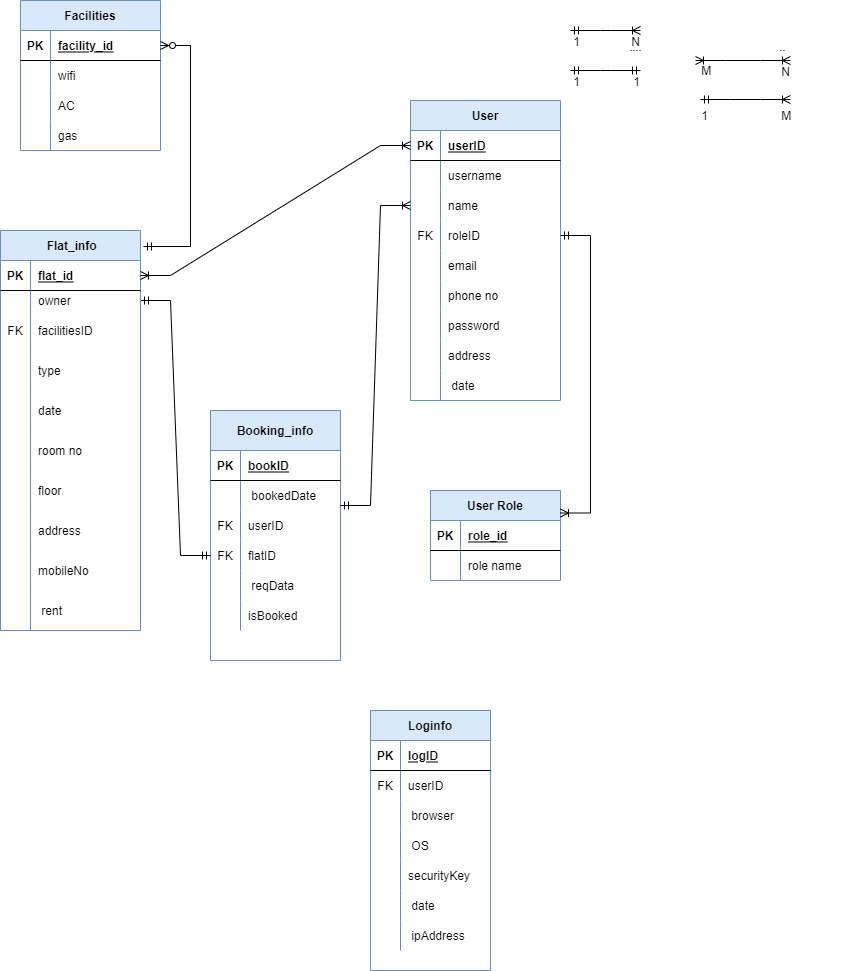
\includegraphics[width=1\textwidth, inner]{images/RM.png}\\
\begin{center}
 Figure-3: Relational modeling
\end{center}
\end{figure}
\clearpage